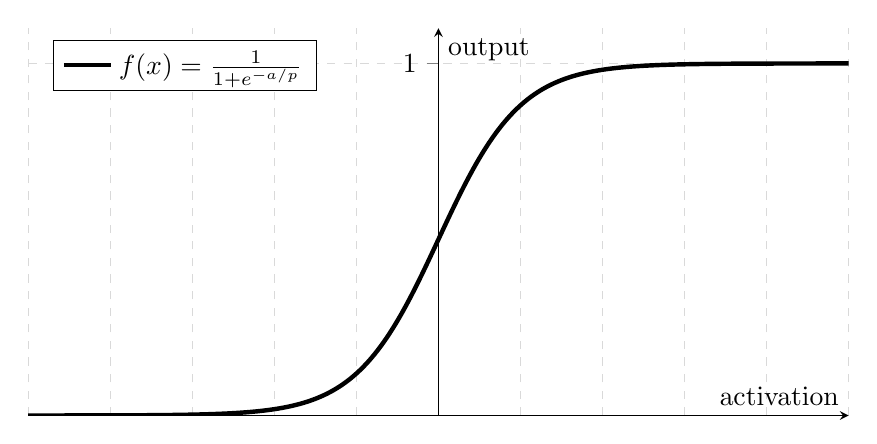
\begin{tikzpicture}
    \begin{axis}[
    	legend pos=north west,
        axis x line=middle,
        axis y line=middle,
        grid = major,
        width=12cm,
        height=6.5cm,
        grid style={dashed, gray!30},
        xmin=-1,xmax= 1,ymin= 0,ymax= 1.1,
        xlabel=activation,ylabel=output,
        tick align=outside,
        ytick={1},
        xmajorticks=false,
        enlargelimits=false]
      \addplot[domain=-1:1, black, ultra thick,samples=500] {1/(1+exp(-10*x))}; 
      \addlegendentry{$f(x)=\frac{1}{1+e^{-a/p}}$}
    \end{axis} 
\end{tikzpicture}